


\begin{table}[h!]
\centering
    \begin{tabular}{|p{0.14\linewidth}|p{0.35\linewidth}|p{0.16\linewidth}|p{0.16\linewidth}|}
    \hline
    \textbf{Symbol} & \textbf{Description} & \textbf{Property} & \textbf{Random}\\[0.5ex]
    \hline
    $T$ & Total time period & $T=n\Delta t$ &No\\
    \hline
    $n$ & Total Number of intervals &  &No\\
    \hline
    $\Delta t$ & One time interval & $\Delta t$=T/n & No\\
    \hline
    $k$ & Number of calls arrived during the time interval (0,$T$) & & Yes\\
    \hline
    $t_i$ & Denotes the time of arrival of each call in interval $(0,T)$ & &Yes\\
    \hline
    $p$ & Probability of receiving a call at time $t_i$ & &No\\
    \hline
    $\lambda$ & Average number of calls $(0,T)$ & $\lambda=np$ &No\\
    \hline
    $e$ & Euler's number & &No\\
    \hline
    \end{tabular}
\end{table}
Lets denote the fixed time interval by [0,$T$].
To find the probability of $k$ number of calls during this time interval, lets divide the interval into $n$ parts of equal length $\Delta t$.
Let us denote the probability of receiving a call at a particular time $t_i$ by $p$. Suppose the telephone exchange receives an average of $\lambda$ calls in time interval of length $T$.\\
Hence, we have
\begin{align}
    np=\lambda\\
    \implies p=\frac{\lambda}{n}
\end{align}
\begin{figure}[ht]
    \centering
    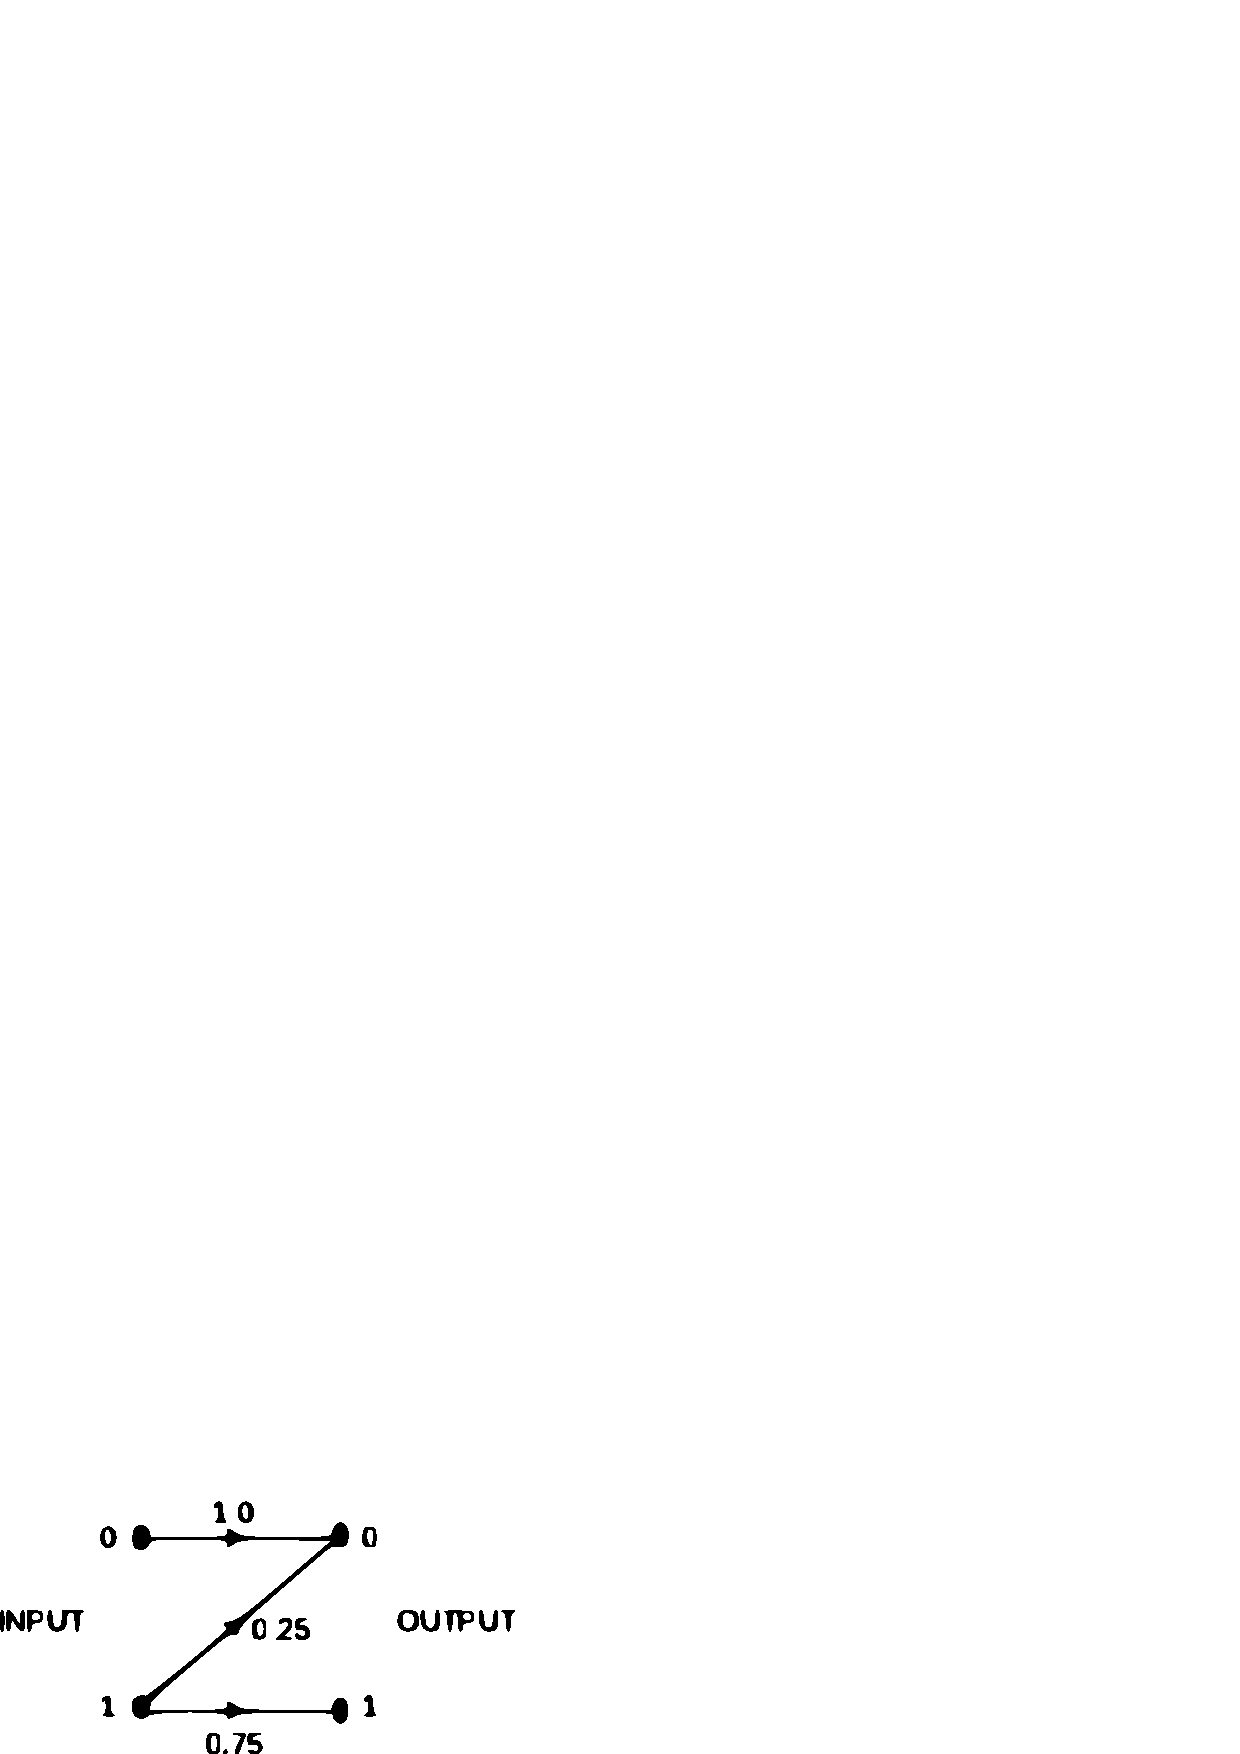
\includegraphics[width=\columnwidth]{solutions/ec/43/Figures/figure1.png}
    \caption{Figure showing division of time intervals}
    \label{ec43:figure_1}
\end{figure}
In Fig. \ref{ec43:figure_1}, the interval (0,$T$) has been divided into n equal parts, where length of each interval is $\Delta t$ and the number of calls in each interval is a random variable.
\begin{figure}[ht]
    \centering
    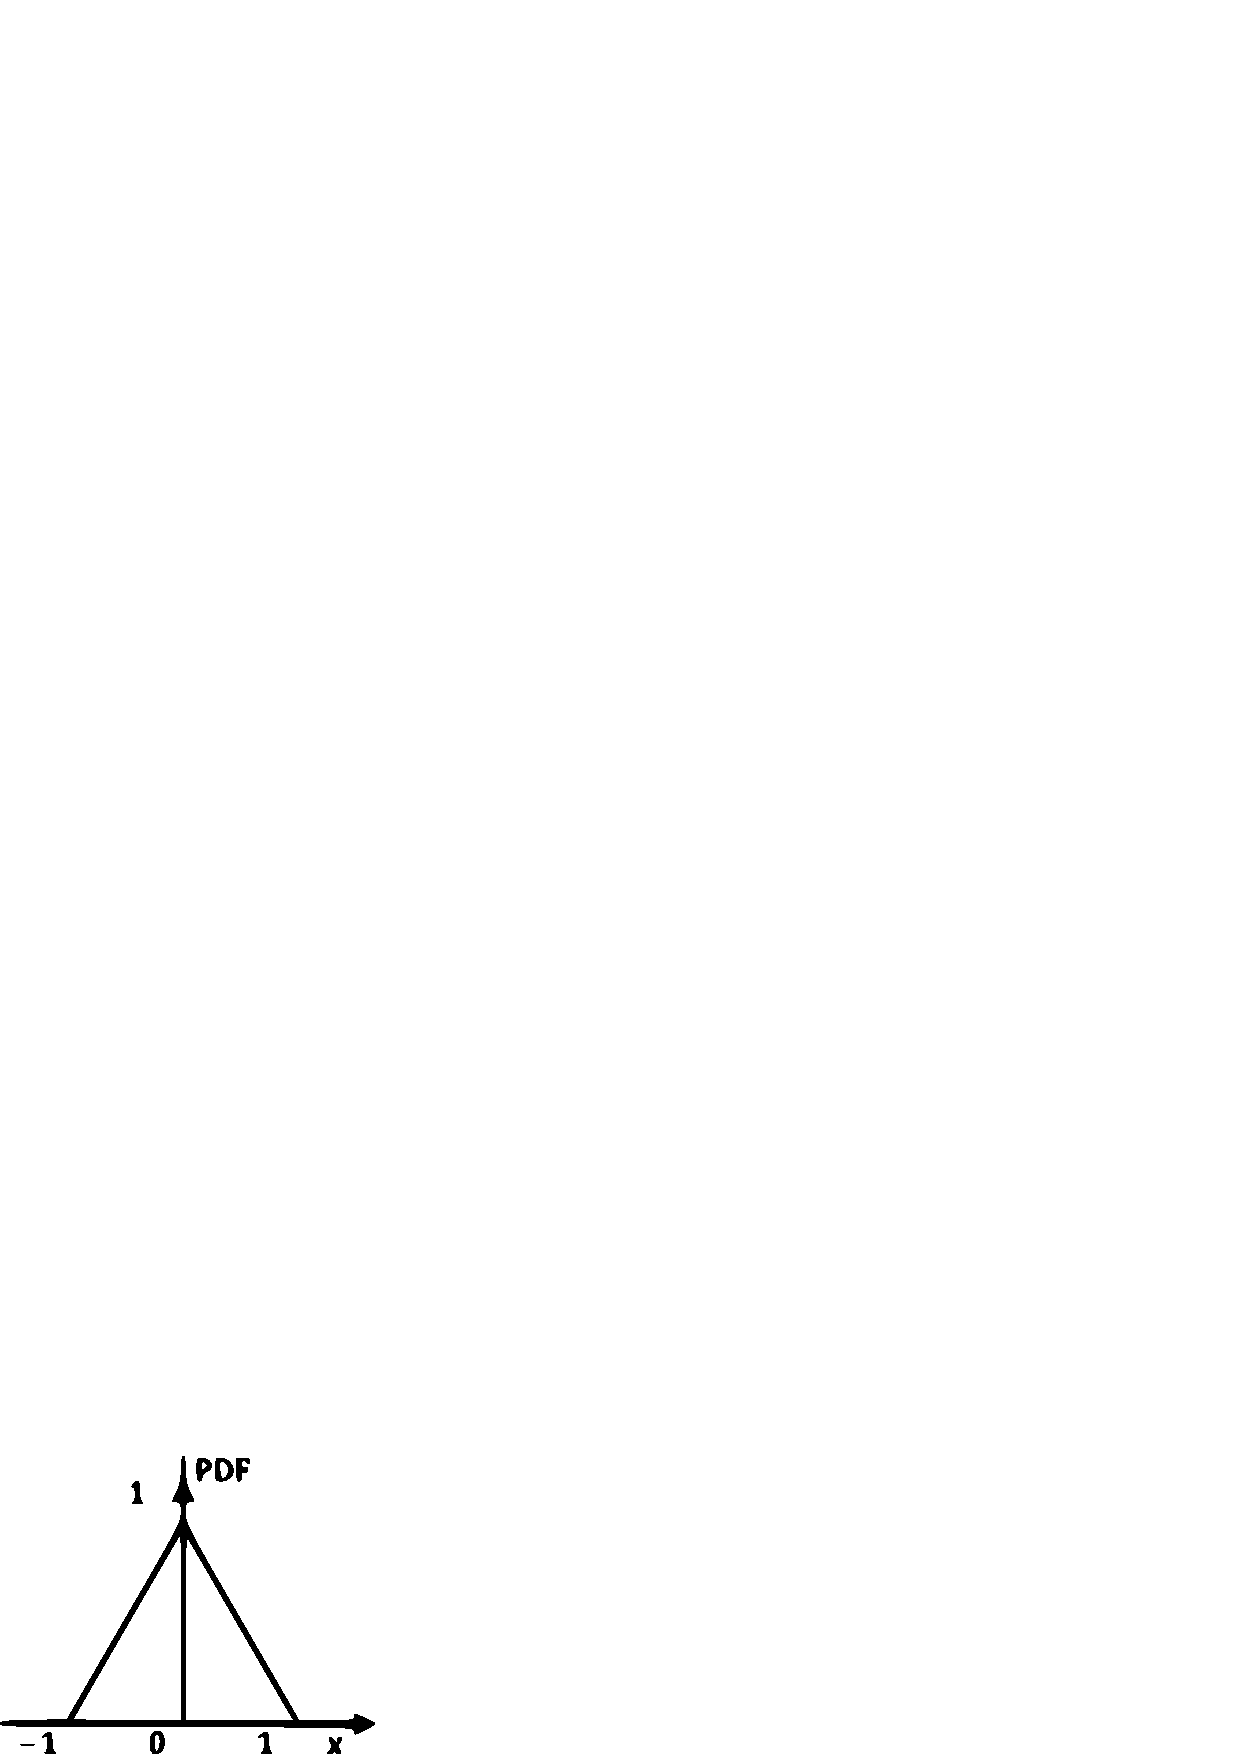
\includegraphics[width=\columnwidth]{solutions/ec/43/Figures/figure2.png}
    \caption{Figure showing times of arrival of $k$ calls}
    \label{ec43:Figure_2}
\end{figure}
$t_i$ where $i=\{1,2,3\cdots k\}$ are the time of arrival of $k$ calls in the interval $(0,T)$.\\

A call has probability $p$ for arriving at $t_i, \forall  i=\{1,2,\cdots k\}$ and the probability of 1-$p$ for not arriving at that instant.\\

In Binomial distribution we have certain number of intervals, i.e. $n$, with probability of arrival of each call as $p$ and for a binomial random variable $X=\{0,1\cdots n\}$, the probability of call arriving in any $k$ intervals is 
\begin{align}
    \pr{X=k}=\comb{n}{k}\cdot p^k\cdot(1-p)^k
\end{align} But in Poisson distribution, we essentially have infinite intervals, so $n\rightarrow\infty$. Thus, the probability expression changes to:
\begin{align}
   \lim_{n \to \infty}\pr{X=k}=\lim_{n \to \infty}\frac{n!}{k!(n-k)!}\left(\frac{\lambda}{n}\right)^k\left(1-\frac{\lambda}{n}\right)^{n-k}
\end{align}
\begin{multline}  \label{ec43:5}
    \lim_{n \to \infty}\pr{X=k}=\\
    \left(\frac{\lambda^k}{k!}\right)\lim_{n \to \infty}\frac{n!}{(n-k)!}\left(\frac{1}{n}\right)^k\left(1-\frac{\lambda}{n}\right)^n\left(1-\frac{\lambda}{n}\right)^{-k}
\end{multline}
Now lets take the limit of right-hand side one term at a time. We’ll do this in three steps. The first step is to find the limit of 
\begin{equation}
\begin{split}\label{ec43:6}
     \lim_{n \to \infty}\frac{n!}{(n-k)!n^k}
     &= \lim_{n \to \infty}\frac{n(n-1)(n-2)..(n-k+1)}{n^k}\\
    & = \lim_{n \to\infty}\left(\frac{n}{n}\right)\left(\frac{n-1}{n}\right)....\left(\frac{n-k+1}{n}\right)\\
   &= \lim_{n \to \infty}\left(1-\frac{1}{n}\right)\left(1-\frac{2}{n}\right)...\left(1-\frac{k-1}{n}\right)\\
    &=1\cdot1\cdot1........1\\
    &=1   
    \end{split}
\end{equation}
Now we have to find the limit of 
\begin{align}\label{ec43:7}
    \lim_{n \to \infty}\left(1-\frac{\lambda}{n}\right)^n 
\end{align}
We know that the definition $e$ is given as 
\begin{align}
    e=\lim_{x \to \infty}\left(1+\frac{1}{x}\right)^x
\end{align}
So, lets replace the value of $-\frac{n}{\lambda}$ by x in \eqref{ec43:7}, we get
\begin{align}\label{ec43:9}
    \lim_{n \to \infty}\left(1-\frac{\lambda}{n}\right)^n =\lim_{x \to \infty}\left(1+\frac{1}{x}\right)^{x(-\lambda)}=e^{-\lambda}
\end{align}
And the third part is to find the limit of 
\begin{align}
    \lim_{n \to \infty}\left(1-\frac{\lambda}{n}\right)^{-k}
\end{align}
As n approaches infinity, this term becomes $1^{-k}$ which is equal to one.
So,
\begin{align}\label{ec43:11}
    \lim_{n \to \infty}\left(1-\frac{\lambda}{n}\right)^{-k}=1
\end{align}
Now on substituting \eqref{ec43:6}, \eqref{ec43:9} and \eqref{ec43:11} in equation \eqref{ec43:5}, we get
\begin{multline}  
    \left(\frac{\lambda^k}{k!}\right)\lim_{n \to \infty}\frac{n!}{(n-k)!}\left(\frac{1}{n}\right)^k\left(1-\frac{\lambda}{n}\right)^n\left(1-\frac{\lambda}{n}\right)^{-k}=\\
    \left(\frac{\lambda^k}{k!}\right)(1)\left(e^{-\lambda}\right)(1)
\end{multline}
This just simplifies into
\begin{align}\label{ec43:final_equation}
    \pr{X=k}=\left(\frac{\lambda^k e^{-\lambda}}{k!}\right)
\end{align}
   \eqref{ec43:final_equation} is equal to probability density function of Poisson distribution, which gives us probability of $k$ successes per period, with given parameter of $\lambda$.\\
   
   $\therefore $The probability distribution function of the total
number of calls in a fixed time interval will be \textbf{Poisson} distribution.\\
Answer: Option(A)

